\section{Appendix}

\subsection{A: Time sheets}

\begin{table}[h]
\begin{tabular}{llllll}
\textbf{Week} & \textbf{think-time} & \textbf{dev-time} & \textbf{xp/analysis-time} & \textbf{write-time} & \textbf{wasted-time} \\ \hline
2             & 2                   & 0                 & 0                         & 0                   & 4                    \\
3             & 3                   & 0                 & 0                         & 2                   & 0                    \\
4             & 3                   & 3                 & 0                         & 0                   & 3                    \\
5             & 1                   & 4                 & 0                         & 0                   & 2                    \\
6             & 1                   & 8                 & 2                         & 3                   & 0                    \\
7             & 1                   & 8                 & 3                         & 2.5                 & 0                    \\
8             & 2                   & 4                 & 4                         & 4                   & 0                    \\
              &                     &                   &                           &                     &                     
\end{tabular}
\end{table}

In the analysis above the hours of the team members are summarized. 
It is clear that in the first two weeks we did not implement anything, but thought more about the system architecture and the possible solutions for the different problems such as consistency and replication.
In the fourth week we started diving in to RMI by reading about RMI and following developer tutorials in order to get familiar with  RMI.
We also started looking in to the provided source code of the DAS system provided on Blackboard and made a start for the implementation.
In the fifth week continued the implementation of the system.
In this week most of the problems (we already explained in the report) were encountered. 
We decided to start a clean implementation again, which is also why our dev-time in the following weeks were quite high.
As explained in the report, we did not have any fancy experiments. 
However, we did test and experiment with the system in other ways as explained.
The time we spend doing so is reported under xp/analysis-time.

NOTE: this table is per person, and the total amount of hours in this table is 102.
Which means that the total for all the members is twice this number.
The amount of hours spend by each member almost the same, which is why we just provided one table.
This is mainly because we scheduled meetings to work on the assignment.

\subsection{B: Metrics}
\begin{figure}[ht]
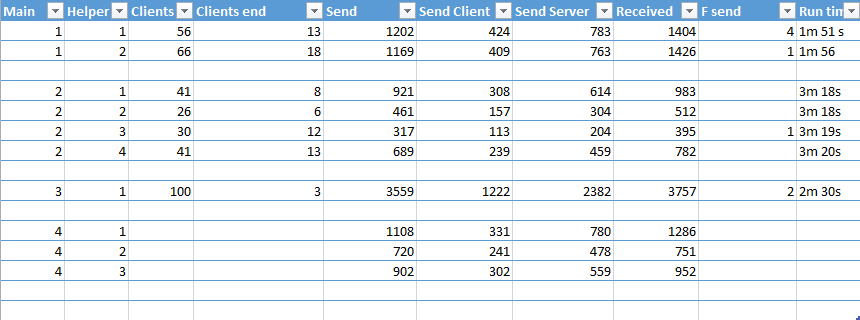
\includegraphics[scale=0.5]{M1.png}
\end{figure}

\begin{figure}[ht]
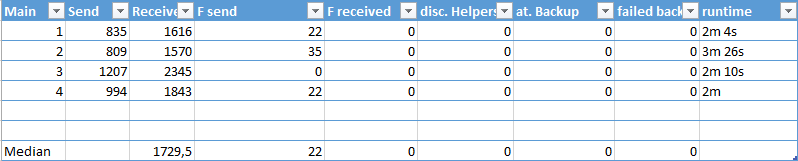
\includegraphics[scale=0.5]{M2.png}
\end{figure}


